%%%%%%%%%%%%%%%%%%%%%%%%%%%%%%%%%%%%%%%%%
% Bellier Rendue court
% Version 1.0 (11/09/2021)
%
% Auteur original:
% Benjamin Bellier
%
% License:
% CC BY-NC-SA 3.0 (http://creativecommons.org/licenses/by-nc-sa/3.0/)
%
% Saved with string encoding Unicode (UTF-8)
%
%%%%%%%%%%%%%%%%%%%%%%%%%%%%%%%%%%%%%%%%%

\documentclass[a4paper, 10pt, twoside]{article}

%----------------------------------------------------------------------------------------
%	    DIFFÉRENTS PACKAGES ET CONFIGURATIONS NÉCESSAIRES
%----------------------------------------------------------------------------------------

\usepackage[round]{natbib} % Parenthèses autour des citations, remplacer par des carrés pour les crochets
\usepackage[french]{babel}
\usepackage[utf8]{inputenc} % Support des caractères avec accents
\usepackage[T1]{fontenc}
\usepackage{lmodern}
\usepackage[pdftex]{graphicx} % Requis pour afficher des images
\usepackage{graphics} % Requis pour afficher des images
\usepackage{color} % Requis pour des couleurs personnalisées
\usepackage{amsmath, amssymb, theorem} % Math packages
\usepackage{listing} % Requis pour inclure des extraits de codes
\usepackage{booktabs} % Requis pour de meilleurs règles horizontales dans les tableaux
\usepackage{xspace} % Fournit la capacité d'utiliser des espace intelligent qui sont utilisé dans \universite et \departement
\usepackage[printonlyused, withpage]{acronym} % inclus une list d'acronymes
\usepackage{rotating} % permet aux tableaux et au figures d'être tourné
\definecolor{couleurliens}{rgb}{0.,0.,0.} % définition de la couleur des liens
\definecolor{couleurliensclickable}{rgb}{0.,0.,0.7}
\usepackage[pdftex,colorlinks=true,urlcolor=couleurliensclickable,linkcolor=couleurliens,citecolor=couleurliens]{hyperref} % Requis pour les liens et changer les options des liens
\usepackage{microtype} % Ajuste légérements l'espacement des polices pour l'esthétique
\usepackage{authoraftertitle} % Requis pour modification de la command \maketitle
\usepackage{datetime} % Requis pour afficher la date dans le document
\usepackage{pdfpages}
\usepackage{listings}
\usepackage[table]{xcolor}
\usepackage{fancyhdr}
\usepackage[absolute]{textpos}

\makeatletter
\renewcommand{\fnum@figure}{\textsc{\figurename~\thefigure}} % Met le texte "Figure 1.1" en capital minuscule
\makeatother

\definecolor{orange}{RGB}{230, 40, 0} % Définition couleur orange
\definecolor{darkblue}{RGB}{0, 0, 30} % Définition couleur bleu foncé

%----------------------------------------------------------------------------------------
%	    INTEGRATION CODE
%----------------------------------------------------------------------------------------

\lstset{
  literate=
  {á}{{\'a}}1 {é}{{\'e}}1 {í}{{\'i}}1 {ó}{{\'o}}1 {ú}{{\'u}}1
  {Á}{{\'A}}1 {É}{{\'E}}1 {Í}{{\'I}}1 {Ó}{{\'O}}1 {Ú}{{\'U}}1
  {à}{{\`a}}1 {è}{{\`e}}1 {ì}{{\`i}}1 {ò}{{\`o}}1 {ù}{{\`u}}1
  {À}{{\`A}}1 {È}{{\'E}}1 {Ì}{{\`I}}1 {Ò}{{\`O}}1 {Ù}{{\`U}}1
  {ä}{{\"a}}1 {ë}{{\"e}}1 {ï}{{\"i}}1 {ö}{{\"o}}1 {ü}{{\"u}}1
  {Ä}{{\"A}}1 {Ë}{{\"E}}1 {Ï}{{\"I}}1 {Ö}{{\"O}}1 {Ü}{{\"U}}1
  {â}{{\^a}}1 {ê}{{\^e}}1 {î}{{\^i}}1 {ô}{{\^o}}1 {û}{{\^u}}1
  {Â}{{\^A}}1 {Ê}{{\^E}}1 {Î}{{\^I}}1 {Ô}{{\^O}}1 {Û}{{\^U}}1
  {œ}{{\oe}}1 {Œ}{{\OE}}1 {æ}{{\ae}}1 {Æ}{{\AE}}1 {ß}{{\ss}}1
  {ű}{{\H{u}}}1 {Ű}{{\H{U}}}1 {ő}{{\H{o}}}1 {Ő}{{\H{O}}}1
  {ç}{{\c c}}1 {Ç}{{\c C}}1 {ø}{{\o}}1 {å}{{\r a}}1 {Å}{{\r A}}1
  {€}{{\EUR}}1 {£}{{\pounds}}1
}

\definecolor{darkWhite}{rgb}{0.96,0.96,0.96}

\lstset{
  aboveskip=3mm,
  belowskip=-2mm,
  backgroundcolor=\color{darkWhite},
  basicstyle=\footnotesize,
  breakatwhitespace=false,
  breaklines=true,
  captionpos=b,
  commentstyle=\color{red},
  deletekeywords={...},
  escapeinside={\%*}{*)},
  extendedchars=true,
  framexleftmargin=16pt,
  framextopmargin=3pt,
  framexbottommargin=6pt,
  frame=tb,
  keepspaces=false,
  keywordstyle=\color{blue},
  language=C,
  literate=
  {²}{{\textsuperscript{2}}}1
  {⁴}{{\textsuperscript{4}}}1
  {⁶}{{\textsuperscript{6}}}1
  {⁸}{{\textsuperscript{8}}}1
  {€}{{\euro{}}}1
  {é}{{\'e}}1
  {è}{{\`{e}}}1
  {ê}{{\^{e}}}1
  {ë}{{\¨{e}}}1
  {É}{{\'{E}}}1
  {Ê}{{\^{E}}}1
  {û}{{\^{u}}}1
  {ù}{{\`{u}}}1
  {â}{{\^{a}}}1
  {à}{{\`{a}}}1
  {á}{{\'{a}}}1
  {ã}{{\~{a}}}1
  {Á}{{\'{A}}}1
  {Â}{{\^{A}}}1
  {Ã}{{\~{A}}}1
  {ç}{{\c{c}}}1
  {Ç}{{\c{C}}}1
  {õ}{{\~{o}}}1
  {ó}{{\'{o}}}1
  {ô}{{\^{o}}}1
  {Õ}{{\~{O}}}1
  {Ó}{{\'{O}}}1
  {Ô}{{\^{O}}}1
  {î}{{\^{i}}}1
  {Î}{{\^{I}}}1
  {í}{{\'{i}}}1
  {Í}{{\~{Í}}}1,
  morekeywords={*,...},
  numbers=left,
  numbersep=10pt,
  numberstyle=\tiny\color{black},
  rulecolor=\color{black},
  showspaces=false,
  showstringspaces=false,
  showtabs=false,
  stepnumber=1,
  stringstyle=\color{gray},
  tabsize=4,
  title=\lstname,
}

%----------------------------------------------------------------------------------------
%	    MISE EN PAGE
%----------------------------------------------------------------------------------------

\usepackage[top=2cm, bottom=2cm, left=2cm, right=2cm]{geometry} % Modifie les marges du document

%----------------------------------------------------------------------------------------
%   EN-TÊTE
%----------------------------------------------------------------------------------------

\pagestyle{fancy}
\fancyhead{}
\renewcommand\headrulewidth{0.4pt}
\fancyhead[CO]{\color{orange} \Large \textbf{Compte-Rendue\\\title}}
\fancyhead[RO]{\scriptsize \color{darkblue} \textit{3\up{ème}~ANNÉE LICENCE INFORMATIQUE}\\
\footnotesize \date\\
\small \bfseries \author}

%----------------------------------------------------------------------------------------
%	   PAGE DE GARDE
%----------------------------------------------------------------------------------------

\renewcommand{\date}{2021-2022}
\renewcommand{\title}{Projet Theatre CEBD}
\renewcommand{\author}{Favre Benjamin\\BELLIER Benjamin}

\begin{document}
%    INSERTION DE L'IMAGE EN HAUT À GAUCHE DE LA PAGE
% -------------------------------------------------------------------------------------------------------------------------------
  \begin{textblock*}{3cm}(1.5cm,4mm)
    \begin{figure}[h]
      \includegraphics[width=2.5cm]{/home/benny/Documents/LaTeX assets/Figures/UFR_IM2AG_2020.jpg}\\[.1cm] % Logo de l'institution
    \end{figure}
  \end{textblock*}
% -------------------------------------------------------------------------------------------------------------------------------
\section*{}
%---------------------------------------------------------------------------------
%    TEXTE
%---------------------------------------------------------------------------------

Lors de ce projet, nous avons utilisé la plateforme github avec le logiciel git,
cliquez sur le lien pour accéder au dépôt du projet~:
\href{https://github.com/BennyBellier/Theatre-CEDB-Project}{https://github.com/BennyBellier/Theatre-CEDB-Project}

\section{Question 1}
  \subsection{Dépendances fonctionnelles}
  Pour établir les dépendances nous nous sommes basés le texte explicatif.\\

  \noindent Pour  les représentations, nous avons trouvées les dépendances fonctionnelles suivantes~:
  \begin{itemize}
    \item noSpec $\rightarrow$ nomSpec, prixBaseSpec
    \item noSpec, dateRep $\rightarrow$ promoRep
    \item PrixBaseRep, promoRep $\rightarrow$ prixRep
  \end{itemize}
  \emph{Commentaire~:}\\
  On constate, qu'il n'y a qu'une seul salle. Donc on trouve la relation :
  dateRep $\rightarrow$ noSpec. Or, on a trouver que la pair (noSpec, dateRep) est une
  clé. Et une partie de la clé ne peut donner l'autre partie de celle-ci.\\

  \noindent Pour les places, nous avons trouvées les dépendances fonctionnelles suivantes~:
  \begin{itemize}
    \item noZone $\rightarrow$ catZone
    \item catZone $\rightarrow$ noZone
    \item noPlace, noRang $\rightarrow$ noZone
  \end{itemize}
  \emph{Commentaire ~:}\\
  On remarque, un doublon, catZone et noZone, qui sont de type différent mais qui indique la même chose.\\

  \noindent Pour les ventes, nous avons trouvées les dépendances fonctionnelles suivantes~:
  \begin{itemize}
    \item noTrans $\rightarrow$ dateTrans, prixTicket, noPlaces, noDossier
    \item noDossier $\rightarrow$ noPlaces, prixTotal
  \end{itemize}
  \emph{Commentaire~:}\\
  Aucune ambiguïtées trouvées.\\

  \noindent Pour les réductions, nous avons trouvées les dépendances fonctionnelles suivantes~:
  \begin{itemize}
    \item dateRep $\rightarrow$ tauxRep
    \item typePers $\rightarrow$ tarifReduit
  \end{itemize}
  \emph{Commentaire~:}\\
  Aucune ambiguïtées trouvées.\\

  \subsection{Normalisation}
  On remarque que, pour la forme normale proposée celle-ci n'excéde pas le 2NF. D'après les dépendances fonctionnelles
  trouvés plus haut. Pour la relation V0\_LesRepresentations, on obtiens un mélange entre une relation et une vue.
  Dans celle-ci est calculé le prix de la représentation (prixRep). De plus, on retrouve par transitivité des boucles~:
  \begin{itemize}
    \item noSpec $\rightarrow$ nomSpec, prixBaseSpec, dateRep, promoRep, prixRep
    \item dateRep $\rightarrow$ promoRep, nomSpec, prixBaseSpec, prixRep
  \end{itemize}
  Quand à la relation V0\_LesPlaces, on trouve des dépendances entres des attributs non clés~:
  \begin{itemize}
    \item noPlace, noRang $\rightarrow$ noZone
    \item noZone $\rightarrow$ catZone, tauxZone
    \item catZone, tauxZone $\rightarrow$ noZone
  \end{itemize}

  Étant donné, que le schéma de relation est obsolète et n'est pas utilisable correctement, nous proposons un nouveau schéma de relation~:\\
  On commence par séparer en deux la relation \emph{V0\_LesRepresentations}~: LesSpectacles et LesRepresentations.\\
  La relation LesSpectacles continent les information concernant un spectacle précis~: son numéro, son nom et son prix de base.
  Quand à la relation LesRepresentations, elle contient les information relative aux dates de représentations des différents spectacles~: date de la représentation,
  numéro du spectacle et la promotion qui est associé à celle-ci.
  On obtient donc les relation suivantes~:\\
  \emph{lesSpectacles}(\textbf{noSpec}, nomSpec, prixBaseSpec),\\
  \emph{LesRepresentations}(\textbf{dateRep}, noSpec, promoRep).\\

\newpage
\thispagestyle{empty}

  \noindent Pour rendre la relation \emph{V0\_LesPlaces} BCNF, on commence par créer la relation
  \emph{LesPlaces}(\textbf{noPlaces, noRang}, noZone). Il reste donc dans \emph{V0\_LesPlaces} les attributs (noZone, catZone, tauxZone).
  Or noZone $\rightarrow$ catZone, tauxZone et catZone, tauxZone $\rightarrow$ noZone. Donc, on créer les relations suivantes~:\\
  \emph{LesZones}(\textbf{noZone}, catZone),\\
  \emph{TypeZones}(\textbf{catZone}, tauxZone).\\

  \noindent On crée ensuite, une relation \emph{lesVentes} qui nous permettras de gérer la vente des palces pour chaque représentations.
  On utilise le principe de panier lors de l'achat d'un ou plusieurs tickets. Donc un dossier sera créé pour chaque ticket ou ensemble de ticket vendue.
  On as donc les relations suivantes~:\\
  \emph{lesVentes}(\textbf{noTrans}, dateTrans, noPlaces, noDossier, PrixTicket),\\
  \emph{LesDossiers}(\textbf{noDossiers}, noPlaces, prixTotal).\\

  \noindent On crée une dernière relation~:
  \emph{LesReductions}(\textbf{typePers}, tarifReduit)\\
  Qui nous permettras de mettre en relation le prix des tickets avec le type de personne qui l'as acheté (ordinaire,
  sénior, militaire, ...).

  On obtients donc le tablleau suivant~:\\[.25cm]
  \begin{tabular}{|c|c|c|c|c|}
    \hline
    \textbf{Relations}&\textbf{1NF}&\textbf{2NF}&\textbf{3NF}&\textbf{BCNF}\\
    \hline
    LesSpectacles&X&X&X&X\\
    \hline
    LesRepresentations&X&X&X&X\\
    \hline
    LesPlaces&X&X&X&X\\
    \hline
    LesZones&X&X&X&X\\
    \hline
    LesVentes&X&X&X&X\\
    \hline
    LesDossiers&X&X&X&X\\
    \hline
  \end{tabular}

\newpage
\thispagestyle{empty}

\section{Question 2}
  \begin{figure}[h]
    \centering
    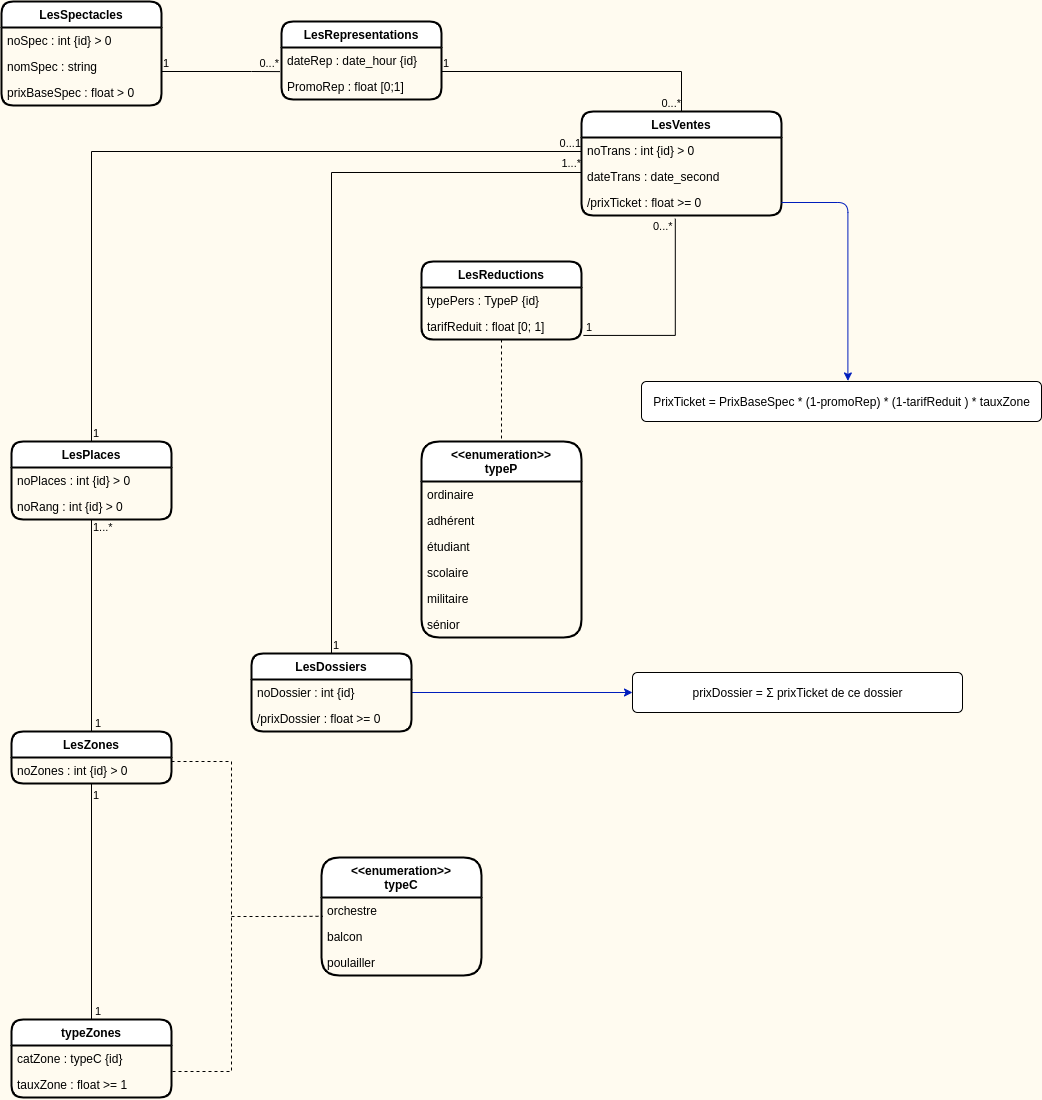
\includegraphics[scale=0.5]{Theatre_UML.png}
  \end{figure}

\section{Question 3}
  \emph{Les attributs en \textbf{gras} sont les clés de la relation.}\\\\
  LesSpectacles (\textbf{noSpec}, nomSpec, prixBaseSpec)\\
  /*<nS, nomS, pBS> $\in$ LesSpectacles $\Longleftrightarrow$ Le spectacle nomS est identifié par le numéro nS et à pour prix de base pBS. */\\\\

\newpage
\thispagestyle{empty}

  LesRepresentations (\textbf{dateRep}, promoRep, noSpec )\\
  /*<dR, prR, nS,> $\in$ LesRepresentations $\Longleftrightarrow$ Une représentation du spectacle numéro nS a lieu a la date dR etfait l'objet d'une promotion prR. */\\\\
  LesVentes (\textbf{noTrans}, dateTrans, PrixTotal, noPlaces, noRang, typeP, noDossier, dateRep)\\
  /*<noT, dT, pT, noP, noR, tP, noD, dR> $\in$ LesVentes $\Longleftrightarrow$ Le numéro de transaction noT possède une date de transaction dT, un numéro de place noP associé a son rang noR. Le prix total de la transaction est calculé en fonction du type de la personne tP, de la potentielle promotion affectée a la représentation qui a lieu a la date dR. Si une vente concerne un seul ticket, celle ci est attribuée a un numéro de dossier noD. Or, si une personne veut effectuer n ventes alors un noD est crée pour ses n ventes. */\\\\
  LesPlaces (\textbf{noPlaces, noRang}, noZone)\\
  /*<noP, noR, noZ> $\in$ LesPlaces $\Longleftrightarrow$ La place noP du rang noR se situe dans la zone noZ. */\\\\
  LesZones (\textbf{noZone}, catZone)\\
  /*<noZ, cZ> $\in$ LesZones $\Longleftrightarrow$ Chaque catégorie cZ est représenté par un numéro de zone noZ dans la salle.*/\\\\
  TypesZones (catZone, tauxZone)\\
  /*<cZ, tZ> $\in$ TypesZones $\Longleftrightarrow$ Chaque taux tZ correspond à une catégorie de zone cZ dans la salle.*/\\\\
  LesDossiers (\textbf{noDossier}, prixDossier)\\
  /*<noD, pD> $\in$ LesDossiers $\Longleftrightarrow$ Le prix du dossier noD est pD. (C'est la somme de toutes les ventes associé au dossier noD. */\\\\
  LesReductions (\textbf{typePers}, tarifReduit)\\
  /*<tP, tR> $\in$ LesReductions $\Longleftrightarrow$ Le tarif réduit tR est réservé au personnes du type tP. */\\\\

  \noindent LesReprésentation[noSpec] $\subseteq$ LesSpectacles[noSpec]~;\\
  LesVentes[dateRep] $\subseteq$ LesRepresentations[dateRep]~;\\
  LesVentes[noPlaces, noRang] $\subseteq$ LesPlaces[noPlace,noRang]~;\\
  LesVentes[typeP] $\subseteq$ LesRéductions[typeP]~;\\
  LesVentes[noD] = LesDossiers[noD]~;\\
  LesPlaces[noZone] $\subseteq$ LesZones[noZone]~;\\
  LesZones[catZone] = TypeZones[catZone]~;\\
  domaine(dateRep) = date(heure) par ex. 24/11/2007 20H~;\\
  domaine(dateTrans) = date(seconde) /\_ par ex. 24/11/2007 19:45:17~;\\
  domaine(typePers) = {’ordinaire’, ’adhérent’, ’étudiant’, ’scolaire’, ’militaire’, ’sénior’}~;\\
  domaine(catZone) = {’orchestre’, ’balcon’, ’poulailler’}~;\\
  domaine(nomSpec) = chaînes de caractères~;\\
  domaine(noZone) = domaine (noPlace) = domaine (noRang) = domaine (noSpec) = doamine(noTrans)\\= entier > 0~;\\
  domaine(prixBaseSpec) = domaine (prixRep) = réels > 0~;\\
  domaine(promoRep) = domaine (tauxZone) = réels dans l’intervalle [0;1].\\

  \noindent Vues possibles~:\\
  LesDossiers car PrixDossier = Somme des prix des tickets correspondant au bon dossier.\\
  Les Ventes car PrixTicket = prix de base du spectacles avec le promotion de ce spectacle, le tarif réduit en fonction de la personne et le taux de la zone.\\
  Salle = pour chaque représentation, le nombre de places disponibles et occupées, et le nom du spectacle correspondant.\\

\end{document}
